\chapter{An overview of Multi-instance learning}\label{chap:MIL}

\name{Multi-instance learning} is an approach to machine learning first described by \cite{dietterich_solving_1997}. In its original form, multi-instance learning (often referred to just as \name{MIL}) was used for \name{supervised learning}, that is to solve problems for which there is already a dataset of known examples and their corresponding labels at the ready. An example of that is in the work \cite{amores_multiple_2013}. The other class of problems solved is \name{unsupervised learning}, where no labels are available in the training phase. Among these is for example \cite{chen_contextual_2012}.

The multi-instance learning paradigm is a type of representation learning on data with some internal structure. While classical machine learning algorithms typically operate on samples represented by a vector of numbers each, MIL relaxes this requirement by representing a sample as a \name{bag} of an arbitrary number of objects. This bag is then treated as one sample -- e.g. in classification, there is a label for the whole bag.

In this chapter, two formalisms for describing multi-instance learning in the context of classification are presented. The algebraic formalism largely consisting of a translation of \cite{dedic_hierarchicke_2017}, where it was first introduced. The stochastic formalism build upon the ideas from \cite{muandet_learning_2012}. Finally, a review of methods for MIL is presented.

\section{Multisets}

In order to properly describe multi-instance learning using the algebraic formalism, a few uncommon definitions are needed.

A multiset is a set allowing repeated elements. Alternatively, it can be seen as an unordered tuple. \cite{knuth_art_1968} formally defines the concept as follows:

\begin{define}
	Let \( \mathset{A} \) be a set and \( m : \mathset{A} \to \mathfield{N} \setminus \left\{ 0 \right\} \). The tuple \( \left( \mathset{A}, m \right) \) is called a \name{multiset} over the set \( \mathset{A} \). For an \( a \in \mathset{A} \), the number \( m \left( a \right) \) is called the \name{multiplicity} (i.e. the number of occurrences) of \( a \). If \( a \in \mathset{A} \), then \( a \) is called an element of \( \left( \mathset{A}, m \right) \) and denoted as
	\[ a \in \left( \mathset{A}, m \right) \]
\end{define}

Obviously, the concept of a multiset is a generalization of the concept of a set and as such, it is usually written as an enumeration its elements, which are repeated as many times as is their multiplicity.

\begin{example}
	The multiset \( \left( \left\{ a, b, c \right\}, \left\{ \left( a, 3 \right), \left( b, 1 \right), \left( c, 5 \right) \right\} \right) \) may be written as \( \left\{ a, a, a, b, c, c, c, c, c \right\} \).
\end{example}

\begin{remark}
	A set can be seen as a special case of a multiset where each element has a multiplicity of 1.
\end{remark}

\begin{define}
	Let \( \mathset{A} \) be a set. A multiset \( \left( \mathset{B}, m \right) \) is called a \name{submultiset} of \( \mathset{A} \) if \( \mathset{B} \subset \mathset{A} \). This is denoted as
	\[ \left( \mathset{B}, m \right) \subset \mathset{A} \]
\end{define}

The previous definition allows for a generalization of the concept of a power set, which is usually denoted as \( \mathcal{P} \left( \mathset{A} \right) \) or \( 2^{\mathset{A}} \).

\begin{define}
	Let \( \mathset{A} \) be a set. A \name{power multiset} of \( \mathset{A} \) is the set
	\[ \mathcal{P}^M \left( \mathset{A} \right) = \left\{ \left( \mathset{B}, m \right) \middle| \left( \mathset{B}, m \right) \text{is a multiset} \wedge \left( \mathset{B}, m \right) \subset \mathset{A} \right\} \]
\end{define}

\begin{remark}
	A power set of \( \mathset{A} \) is sometimes expressed as the set of all function from \( \mathset{A} \) to \( \left\{ 0, 1 \right\} \), written as \( \left\{ 0, 1 \right\}^{\mathset{A}} \). \( \left\{ 0, 1 \right\} \) coincides with the von Neumann ordinal 2, therefore the power set is often denoted \( 2^{\mathset{A}} \). Similarly, the power multiset may be expressed as the set of all functions from \( \mathset{A} \) to \( \mathfield{N} \) (where \( 0 \in \mathfield{N} \)). It is therefore possible to use an analogous notation \( \mathcal{P}^M \left( \mathset{A} \right) = \mathfield{N}^\mathset{A} \). This analogy extends to the size of the sets in question where
	\[ \left\lvert 2^{\mathset{A}} \right\rvert = 2^{\left\lvert \mathset{A} \right\rvert} \qquad \text{and} \qquad \left\lvert \mathfield{N}^\mathset{A} \right\rvert = + \infty \]
	for all \( \mathset{A} \neq \emptyset \).
\end{remark}

\begin{define}
	Let \( \mathset{B} = \left( \mathset{A}, m \right) \) be a multiset where \( \mathset{A} \) is finite. The cardinality of the multiset \( \mathset{B} \) is
	\[ \left\lvert \mathset{B} \right\rvert = \sum_{a \in \mathset{A}} m \left( a \right) \]
\end{define}

The summation of two multisets can be easily defined as follows.

\begin{define}\label{def:multiset-sum}
	Let \( \mathset{B}_1 = \left( \mathset{A}_1, m_1 \right) \) and \( \mathset{B}_2 = \left( \mathset{A}_2, m_2 \right) \) be two multisets. Then the sum of \( \mathset{B}_1 \) and \( \mathset{B}_2 \) is
	\[ \mathset{B}_1 \oplus \mathset{B}_2 = \left( \mathset{A}_1 \cup \mathset{A}_2, m \right) \]
	where
	\[ m \left( a \right) = \begin{cases}
			m_1 \left( a \right) &\text{for} \quad a \in \mathset{A}_1 \setminus \mathset{A}_2 \\
			m_2 \left( a \right) &\text{for} \quad a \in \mathset{A}_2 \setminus \mathset{A}_1 \\
			m_1 \left( a \right) + m_2 \left( a \right) &\text{for} \quad a \in \mathset{A}_1 \cap \mathset{A}_2 \\
		\end{cases} \]
\end{define}

\section{An algebraic formalism for multi-instance learning}
Multi-instance learning (see \cite{dietterich_solving_1997}) in its original form is an approach to representing and solving problems where there exist samples from a space \( \mathspace{X} \) and their corresponding labels from a space \( \mathspace{Y} \) (the labels are also often called classes) and the goal is to find a mapping of samples to labels which correctly predicts the targets on the data. Unlike classical supervised learning, there is no known solution consisting of pairs of samples and labels. Instead, the samples are grouped together into so-called bags, which are defined as follows:

\begin{define}
	Let \( \mathspace{X} \) be a set of samples. Then the \name{bag space} is a multiset \( \mathspace{B} \) with the properties
	\begin{enumerate}
		\item \( \mathspace{B} \subset \mathcal{P}^M \left( \mathspace{X} \right) \)
		\item \( \left( \forall x \in \mathspace{X} \right) \left( \exists B \in \mathspace{B} \right) \left( x \in B \right) \)
	\end{enumerate}
	Elements of the bag space are called \name{bags}.
\end{define}

Multi-instance learning classification uses a dataset consisting of pairs of bags and labels to learn a mapping between them. \cite{dietterich_solving_1997} provides the following example of a multi-instance problem:

\begin{example}
	Suppose there is a keyed lock on the door to the supply room in an office. Each staff member has a key chain containing several keys. One key on each key chain can open the supply room door. For some staff members, their supply room key opens only the supply room door; while for other staff members, their supply room key may open one or more other doors (e.g., their office door, the mail room door, the conference room door).

	Suppose you are a lock smith and you are attempting to infer the most general required shape that a key must have in order to open the supply room door. If you knew this required shape, you could predict, by examining any key, whether that key could unlock the door. What makes your lock smith job difficult is that the staff members are uncooperative. Instead of showing you which key on their key chains opens the supply room door, they just hand you their entire key chain and ask you to figure it out for yourself! Furthermore, you are not given access to the supply room door, so you can’t try out the individual keys. Instead, you must examine the shapes of all the keys on the key rings and infer the answer.
\end{example}

In this example, the keys (or, more precisely their descriptions by feature vectors) are the samples from \( \mathspace{X} \). The key chains are bags. Even though it makes sense to ask for each key whether it unlocks the supply room, this information is not provided. Instead, only a key-chain-level information is available. On the other hand, it may be stated that a key chain opens the supply room door if and only if it contains a key which opens the door. This naturally leads to the following definition:

\begin{define}\label{def:baglabel}
	Let \( \mathspace{X} \) be an sample space and \( \mathspace{Y} \) a label space such that
	\[ \left( \forall x \in \mathspace{X} \right) \left( \exists_1 y_x \in \mathspace{Y} \right) \]
	Let \( \mathspace{B} \) be a bag space. Let maximum be well-defined in \( \mathspace{Y} \). Then the label of the bag \( B \in \mathspace{B} \) is
	\[ y_B = \max_{x \in B} \left( y_x \right) \in \mathspace{Y} \]
\end{define}

As will later be shown in sections \ref{sec:bag-space-paradigm} and \ref{sec:embedded-space-paradigm}, this isn't the only interpretation of multi-instance learning. There are problems where the instance-level labels are not only no known, but even not well-defined as the bag isn't seen as a mere collection of objects but as a distinct object of its own.

\section{A stochastic formalism for multi-instance learning}\label{sec:stochastic-formalism}
An alternative formalism for multi-instance learning was first introduced in \cite{pevny_using_2017}. This formalism builds on the previous work \cite{muandet_learning_2012}, which presents the following formalism for learning from distributions:

Let for the space \( \mathspace{X} \) exist a measurable space \( \left( \mathspace{X}, \mathspace{A} \right) \), where \( \mathspace{A} \) is a \( \sigma \)-algebra of \( \mathspace{X} \). Let \( \mathcal{P}^\mathspace{X} \) denote the set of all probability measures on \( \left( \mathspace{X}, \mathspace{A} \right) \). The goal of is to learn a function \( h : \mathcal{P}^{\mathspace{X}} \to \mathspace{Y} \) from a set of example pairs \( \left\{ \left( P_i, y_i \right) \right\} \) where \( P_i \in \mathcal{P}^\mathspace{X} \) and \( y_i \in \mathspace{Y} \). In order to be able to efficiently learn from distributions, an embedding of the distribution as a mean function \( \mu \) is introduced. Let \( \mathspace{H} \) be a reproducing kernel Hilbert space of functions \( f : \mathspace{X} \to \mathfield{R} \) with a reproducing kernel \( k : \mathspace{X} \times \mathspace{X} \to \mathfield{R} \). The mean map \( \mu : \mathcal{P}^\mathspace{X} \to \mathspace{H} \) is defined as
\[ \mu \left( P \right) = \int_\mathspace{X} k \left( x, \cdot \right) \mathrm{d}P \left( x \right) \]
Let \( \mu_P = \mu \left( P \right) \) for all \( P \in \mathcal{P}^\mathspace{X} \). Then
\[ \mathbb{E}_P \left[ f \right] = \Braket{\mu_p, f}_\mathspace{H} \]

Given \( m \) training samples of the form \( \left( P_i, y_i \right) \in \mathcal{P}^\mathspace{X} \times \mathfield{R} \) and a loss function \( L : \left( \mathcal{P}^\mathspace{X} \times \mathfield{R}^2 \right)^m \to \mathfield{R} \cup \left\{ +\infty \right\} \), the goal can be formulated as the task of finding a \( f \in \mathspace{H} \) minimizing the risk functional
\[ L \left( P_1, y_1, \mathbb{E}_{P_1} \left[ f \right], \dots, P_m, y_m, \mathbb{E}_{P_m} \left[ f \right] \right) \]

Given this general formalism, the extension to multi-instance learning is fairly straightforward. A bag \( B \) is viewed as a set of realizations of a particular probability distribution \( P \in \mathcal{P}^\mathspace{X} \), that is
\[ B = \left\{ x_i \middle| x_i \sim P, i \in \left\{ 1, \dots, m \right\}, m \in \mathfield{N} \right\} \]
A core assumption of this formalism is that \( P = P \left( P_B, y_B \right) \) where \( P_B \) is the probability distribution of instances in the bag \( B \) and \( y_B \) is the label assigned to \( B \). That is, the probability distribution of the bag is dependent on its assigned label.

In order to define a kernel function on bags (which will be needed in section \ref{sec:bag-space-paradigm}), the mean map \( \mu \) is associated with the kernel \( K : \mathcal{P}^\mathspace{X} \times \mathcal{P}^\mathspace{X} \to \mathfield{R} \) defined as
\[ K \left( P, Q \right) = \Braket{\mu_P, \mu_Q}_\mathspace{H} = \int_\mathspace{X} \int_\mathspace{X} k \left( x, y \right) \mathrm{d}P \left( x \right) \mathrm{d}Q \left( y \right) \]

\section{Approaches to solving multi-instance problems}
In this section, there are described the three major approaches to solving multi-instance classification problems. The section is sourced primarily from \cite{pevny_using_2017} and \cite{pevny_discriminative_2016}.

\subsection{Instance-space paradigm}
Instance-space paradigm is the original approach proposed by \cite{dietterich_solving_1997}. The existence of labels on the level of instances is presumed, even though such labels aren't known even in the training phase. The goal of this approach is to model the unknown instance-level labelling as \( f : \mathspace{X} \to \mathspace{Y} \) and use it to compute the bag-level label analogically to definition \ref{def:baglabel}, that is
\[ y_B = \max_{x \in B } \left( f \left( x \right) \right) \]

There are many applications of instance-space paradigm, the most important of which are described next. (Also see \cite{andrews_support_2002} \cite{zhang_multiple_2006})

\name{BP-MIP}, proposed by \cite{zhou_neural_2002}, is an application of multi-instance learning to binary classification, i.e. \( \mathspace{Y} = \left\{ -1, +1 \right\} \). A feedforward neural network is used, its output for the \( j \)-th instance of the \( i \)-th bag denoted \( o_{ij} \). An instance-level error function is defined as
\[ E_{ij} = \begin{cases}
		0 &\text{for} \quad y_{B_i} = -1 \wedge o_{ij} < 0.5 \\
		0 &\text{for} \quad y_{B_i} = +1 \wedge o_{ij} \geq 0.5 \\
		\frac{1}{2} \left( o_{ij} - 0.5 \right)^2 &\text{otherwise}
	\end{cases} \]
This instance-level error function is then used to compute the bag-level error function as \footnote{The original article erroneously states the upper bound as \( \left\lvert b_j \right\rvert \)}
\[ E_i = \begin{cases}
		\max_{1 \leq j \leq \left\lvert B_i \right\rvert} E_{ij} &\text{for} \quad y_{B_i} = -1 \\
		\min_{1 \leq j \leq \left\lvert B_i \right\rvert} E_{ij} &\text{for} \quad y_{B_i} = +1
	\end{cases} \]
And this is in turn used to compute the global loss function
\[ E = \sum_{i = 1}^{\left\lvert \mathspace{B} \right\rvert} E_i \]
With such a well-defined global loss function, the back-propagation algorithm can be used with a slight modification described in the original article.

\name{EM-DD}, proposed by \cite{zhang_em-dd:_2002}, combines the \name{expectation-maximization} algorithm (see \cite{dempster_maximum_1977}) with the \name{diverse density} algorithm (see \cite{maron_framework_1998}). The EM-DD algorithm starts with a target hypothesis \( h \in \mathspace{Y} \), which is then refined with the EM algorithm. In the E-step, the instance thought to be most responsible for the label of each bag is picked. In the M-step, the gradient ascent algorithm is used to find a new hypothesis \( h' \) which maximizes \( \mathrm{DD} \left( h \right) \). \( \mathrm{DD} \left( h \right) \) corresponds to the likelihood that \( h \) is the actual target. These steps are then repeated, refining the hypothesis.

\subsection{Bag-space paradigm}\label{sec:bag-space-paradigm}
The bag-space paradigm is a formalism in which the notion of instance-level labels is abandoned (that is, the labels are presumed to not only be unknown, but even undefined) and only bag-level labels are assumed to exist. The definition \ref{def:baglabel} is no longer used, so some other way of working with bags must be devised. In order to do this, a bag distance function or a bag kernel function is defined, having the form
\[ k : \mathspace{B} \times \mathspace{B} \to \mathfield{R}_0^+ \]
Because the notion of an instance-level label is no longer used, the sought classification function is of the form \( f : \mathspace{B} \to \mathspace{Y} \).

\name{Citation-kNN}, proposed by \cite{wang_solving_2000}, defines a modified Hausdorff distance for bags \( B_1, B_2 \in \mathspace{B} \) as
\[ H \left( B_1, B_2 \right) = \min_{x \in B_1} \min_{y \in B_2} \left\lVert x - y \right\rVert \]
The \( k \)-nearest neighbour algorithm (see \cite{dasarathy_nearest_1991}) is modified for this application by adding a system of \name{citations} and \name{references}. The \( r \)-nearest references are the nearest neighbours from the vanilla kNN algorithm and the \( c \)-nearest citers are defined as
\[ \mathrm{Citers} \left( x, c \right) = \left\{ x_i \middle| \mathrm{Rank} \left( x_i, x \right) \leq c \wedge x_i \in B \right\} \]
For each bag, the \( r \)-nearest references and the \( c \)-nearest citers are found using the modified Hausdorff distance. If among those there are more positive bags than there are negative ones, the bag is labelled as positive. Otherwise, the bag is labelled as negative.

For more applications using the bag-space paradigm, see \cite{wang_solving_2000}, \cite{kwok_marginalized_2007}, \cite{gartner_multi-instance_2002}, \cite{haussler_convolution_1999}, \cite{zhou_multi-instance_2008} and \cite{muandet_learning_2012}.

\subsection{Embedded-space paradigm}\label{sec:embedded-space-paradigm}
In the embedded space paradigm, labels are only defined on the level of bags, same as in the bag-space paradigm. In order for these bag labels to be learned, an embedding function of the form \( \phi : \mathspace{B} \to \bar{\mathspace{X}} \) must be defined, where \( \bar{\mathspace{X}} \) is a latent space, which may or may not be identical to \( \mathspace{X} \). Using this function, each bag can be represented by an object \( \phi \left( B \right) \in \bar{\mathspace{X}} \), which makes it possible to use any off-the-shelf supervised learning algorithm acting on \( \bar{\mathspace{X}} \). Among the simplest embedding functions are e.g. element-wise minimum, maximum and mean. A more complicated embedding function may for example apply a neural network to each instance of the bag and subsequently pool the instances using one of the aforementioned functions.

\name{MILES}, proposed by \cite{chen_miles:_2006}, uses an instance dictionary \( \mathspace{D} \) to define an embedding function representing the degree of similarity between the bag and the dictionary, that is
\[ \phi : \mathspace{B} \to \mathfield{R}^{\left\lvert \mathspace{D} \right\rvert} \]
which is defined element-wise as
\[ \phi_i \left( B \right) = \sum_{x \in B} k \left( x, d_i \right) \quad \text{where} \quad d_i \in \mathspace{D} \]
where
\[ k \left( x, d \right) = \begin{cases}
		\exp \left( - \frac{1}{\sigma^2} \left\lVert x - d \right\rVert^2 \right) &\text{if } d \text{ is the nearest neighbour of } x \text{ in } \mathspace{D} \\
		0 &\text{otherwise}
	\end{cases} \]
The dictionary is populated by a 1-class support vector machine (see \cite{zhu_1-norm_2004}), which, however, has a high computational complexity.

\cite{pevny_nested_2020} and \cite{dedic_hierarchicke_2017} present an approach to learning to classify HTTP traffic by utilizing sets of URLs. The structure of the data is highly exploited using the embedded-space paradigm. The approach is innovative in that it uses multiple layers of MIL nested in each other -- that is the instances of a bag do not necessarily need to be feature vectors, but can be bag in themselves. The HTTP traffic of a particular client is therefore represented as a bag of all second-level domains the client has exchanged datagrams with. Each second-level domain is then represented as a bag of individual URLs which the client has connected to. Individual URLs are then split into 3 part, domain, path and query, and each part is represented as a bag of tokens, which can then be broken down eve further. The model is shown in figure \ref{fig:HTTP-paper}. In the end, the model consists of 5 nested MIL problems.

\begin{figure}
	\centering
	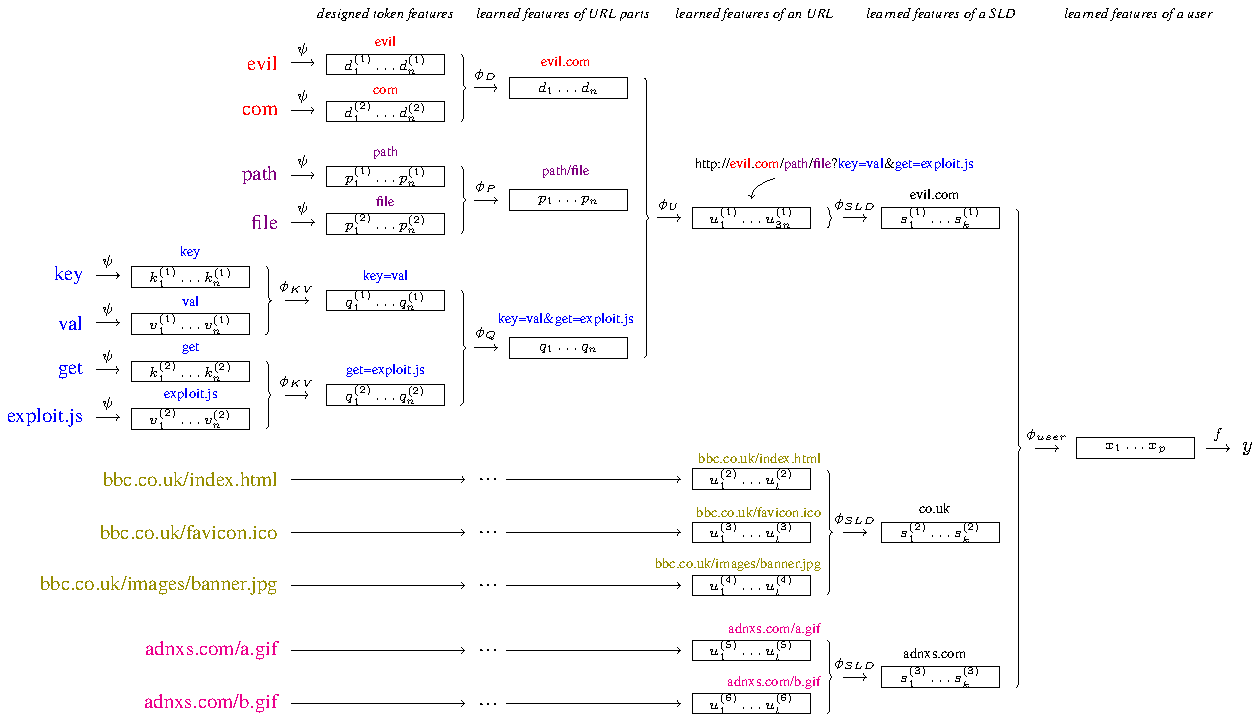
\includegraphics[width=\textwidth]{images/HTTP-paper/HTTP-paper.pdf}
	\caption{Hierarchical model of the network traffic of a single computer. The computer is modelled by a set of remote servers and each remote server is modelled by a set of messages (connections) from the given computer to it. Figure from \cite{pevny_nested_2020}.}\label{fig:HTTP-paper}
\end{figure}

An added benefit of MIL is also in its relatively easy explainability and interpretability. \cite{pevny_nested_2020} present a way to extract indicators of compromise and explain the decision using the learned MIL model.

For more applications using the embedded-space paradigm, see \cite{cheplygina_multiple_2015}, \cite{chen_image_2004} \cite{foulds_learning_2008} and \cite{zhang_multi-instance_2009}.

\subsection{A comparison of the approaches}
For this work, the embedded-space paradigm was chosen. The main reason for this is the development multi-instance learning has gone through since its inception. In the pioneering work of \cite{dietterich_solving_1997}, it is assumed that a bag is just a convenient collection of instances which could be used directly, but have no available per-instance labels. This notion of MIL has, however, since evolved beyond these simple cases and the instance-space paradigm is no longer suitable. The previous work \cite{pevny_nested_2020} presents a clear example where multi-instance learning is used as a general toolkit for learning representations from structured data and even defines how to use nested MIL problems to represent complex hierarchical structures. To this end, the embedded space paradigm is used in this work as it is the only one for which such a structured, multi-layered approach has been proposed.

The bag-space paradigm has clear prior art in the domain of clustering. For large datasets, however, this approach is not feasible due to its high computational complexity. This presents another argument in favor of using the embedded-space paradigm, as the target application of this work is in a domain with extremely large datasets.
